\chapter{Ideal Fluids}

We'll start our exploration of solutions to the Navier-Stokes equation with \emph{ideal fluids}, which we'll define as 
\begin{enumerate}
\item having no viscosity, and
\item having constant density (incompressible).
\end{enumerate}
Of course, \emph{real} fluids always have \emph{some} viscosity; however, as discussed in Section \ref{sec_viscosity}, in some cases an ideal fluid can be a good approximation to a real one.  Keep in mind, however, that the boundary layer present in viscous fluids can never be described by an ideal fluid, so we'll miss some of the physics due to that.

Under these assumptions, the Navier-Stokes equation is usually called \emph{Euler's equation},
\begin{equation}
\label{eq_euler}
\boxed{
\frac{D \uu}{Dt} = -\frac{1}{\rho} \grad p + \mathbf{g}.
}
\end{equation}
The incompressibility condition,
\begin{equation}
\div \uu = 0,
\end{equation}
remains the same.





\section{Static Fluids}

The simplest solution to either the Navier-Stokes equation or Euler's equation is the trivial one:  suppose the fluid is at rest, so that $\uu = 0$ everywhere.  Then Euler's equation reduces to 
\[
0 = -\frac{1}{\rho} \grad p + \mathbf{g},
\]
or 
\[
\grad p = \rho \mathbf{g}.
\]
If we take the direction of gravity to be down, so that $\mathbf{g} = [0,0,-g]$, this equation says
\[
\frac{\partial p}{\partial x} = 0, \quad \frac{\partial p}{\partial y} = 0, \quad \frac{\partial p}{\partial z} = -\rho g.
\]
The first two equations just say that the pressure $p$ doesn't depend explicitly on $x$ or $y$, and we can integrate the third to get
\begin{equation}
p = p_0 - \rho g z,
\end{equation}
where $p_0$ is the integration constant.  If our fluid has a ``free surface'' -- it's open to the atmosphere -- at $z=0$, then $p_0$ is the atmospheric pressure.

This result is simple and tells us what we pretty much know:  as you go down in depth ($z < 0$) in a fluid, the pressure increases.  Note, however, that we've assumed the density $\rho$ stays constant; in some fluids (like the atmosphere) it's a bad assumption, while in others (like the ocean, at least for reasonable depths) it's okay.






\section{Bernoulli's Principle}

For our next result, we'll first need to rewrite Euler's equation.  Since gravity is a conservative force, we can always write it in terms of the gradient of a scalar, so that
\[
\mathbf{g} = - \grad \chi,
\]
where $\chi$ is the gravitational potential.  For example, setting $\chi = gz$ gives us our usual $\mathbf{g}$ pointing down along the $z$ axis.

With this change, Euler's equation becomes
\[
\frac{\partial \uu}{\partial t} + (\uu \cdot \grad) \uu = -\grad \left( \frac{p}{\rho} + \chi \right).
\]
It turns out that the second term on the left can be written as (see Problem \ref{prob_vc3})
\begin{equation}
 (\uu \cdot \grad) \uu = (\curl \uu ) \times \uu + \grad (\tfrac{1}{2} \uu^2).
\end{equation}
Note that I've written $\uu^2$ for $\uu \cdot \uu$; as usual, be careful of all the different $u$'s we deal with.  With this substitution, and moving the gradient onto the right hand side, Euler's equation is now
\begin{equation}
\frac{\partial \uu}{\partial t} + (\curl \uu ) \times \uu = -\grad \left( \frac{p}{\rho} + \tfrac{1}{2} \uu^2 + \chi \right).
\end{equation}

This doesn't look any better than the original form of Euler's equation, though.  We can clean it up a bit by defining
\[
H \equiv \frac{p}{\rho} + \tfrac{1}{2} \uu^2 + \chi,
\]
which is sometimes called the ``total head'' or ``energy head'' of the flow.  If we also assume the flow is \emph{steady}, we then have
\begin{equation}
(\curl \uu ) \times \uu = -\grad H.
\label{eq_bernoulli}
\end{equation}
One last step -- take the dot product with $\uu$ for both sides:
\[
\uu \cdot [(\curl \uu ) \times \uu] = -\uu \cdot \grad H.
\]
But now the left hand side is zero -- the term in the square brackets has a direction perpendicular to $\uu$, so the dot product with $\uu$ vanishes.  

So we're left, finally, with Bernoulli's streamline theorem, which says that, for steady flow,
\begin{equation}
\boxed{
(\uu \cdot \grad) H  = 0.
}
\end{equation}
This means that $H$ is \emph{constant along a streamline} for steady flow.

If the fluid is also irrotational, so that $\curl \uu = 0$, equation (\ref{eq_bernoulli}) gives us the stronger statement
\begin{equation}
\boxed{
\grad H = 0,
}
\end{equation}
so that $H$ is constant everywhere in the fluid.

\begin{example}[A leaky bucket]
A large tank of water, open to the atmosphere at the top, suddenly springs a leak near the bottom (see Figure \ref{fig_leaky_bucket}).  If the hole is 1.0 m below the free surface, what is the speed of the water as it comes out the hole?

\begin{figure}
\centering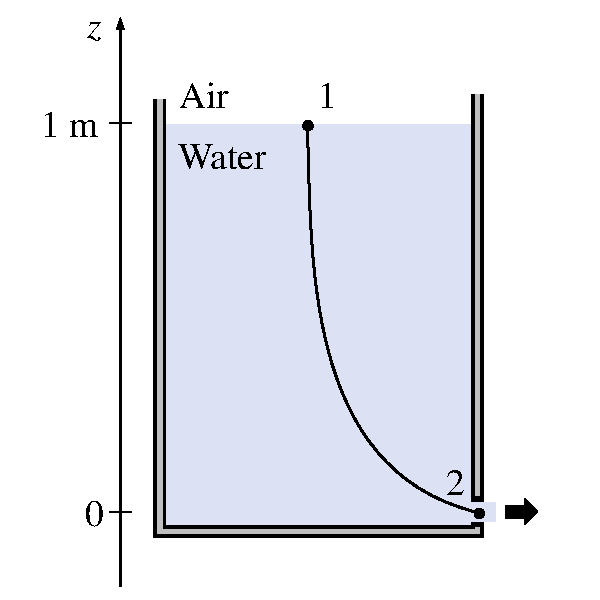
\includegraphics[width=0.5\linewidth]{Figures/Chapter3/fig_leaky_bucket}
\caption{A large tank of water has sprung a leak.  How fast is the water moving as it comes out of the hole?}
\label{fig_leaky_bucket}
\end{figure}


This is a good case for Bernoulli's principle, since the flow is (approximately) steady -- the surface will drop only slowly if the hole is small.  We can therefore use the streamline theorem:
\[
H = \frac{p}{\rho} + \tfrac{1}{2} \uu^2 + gz = \text{constant}.
\]
Presumably there exists a streamline that connects the free surface at the top of the tank with the hole (joining points 1 and 2 as shown in Figure \ref{fig_leaky_bucket}).  Then we can evaluate $H$ at both points:
\begin{itemize}
\item Point 1 $\to H_1 = \frac{p_1}{\rho} + \tfrac{1}{2} \uu_1^2 + gz_1$
\item Point 2 $\to H_2 = \frac{p_2}{\rho} + \tfrac{1}{2} \uu_2^2 + gz_2$
\end{itemize}
But $p_1 = p_2 = p_0$ since both locations are open to the atmosphere.  We'll also take $\uu_1 = 0$, since the surface drops only very slowly.  Finally, using the coordinate system shown in Figure \ref{fig_leaky_bucket}, we have $z_2 = 0$ (and $z_1 = 1$ m).

Setting $H_1 = H_2$ then gives us
\[
\frac{p_0}{\rho} + gz_1 = \frac{p_0}{\rho} + \tfrac{1}{2} \uu_2^2.
\]
The pressure terms cancel, and we can rearrange for the speed of the water:
\[
|\uu| = \sqrt{2gz_1} \approx 4.4 \text{ m/s}.
\]
\end{example}









\section{The Vorticity Equation}
\label{sec_vorticity_eq}

Let's rewrite Euler's equation again, this time in terms of the vorticity.  Going back to equation (\ref{eq_bernoulli}) and writing $\vort = \curl \uu$, we have
\[
\frac{\partial \uu}{\partial t} + \vort \times \uu = -\grad H.
\]
Take the curl of both sides:
\[
\frac{\partial \vort}{\partial t} + \curl (\vort \times \uu) = -\curl \grad H.
\]
But the curl of a gradient is identically zero (see Problem \ref{prob_vc2}), so the right hand side vanishes.

Now, there's a vector identity (another one!) that says, for two vectors $\mathbf{F}$ and $\mathbf{G}$, that
\begin{equation}
\curl (\mathbf{F} \times \mathbf{G}) = (\mathbf{G} \cdot \grad) \mathbf{F} - (\mathbf{F} \cdot \grad) \mathbf{G} + \mathbf{F} (\div \mathbf{G}) - \mathbf{G} (\div \mathbf{F})
\end{equation}
(see Problem \ref{prob_vc4}).  Using this in the equation above, with $\mathbf{F} \to \vort$ and $\mathbf{G} \to \uu$, gives us
\[
\frac{\partial \vort}{\partial t} + (\uu \cdot \grad) \vort - (\vort \cdot \grad)\uu + \vort (\div \uu) - \uu(\div \vort) = 0.
\]
Of course, we're dealing with an ideal fluid, so $\div \uu = 0$, and, since $\vort$ is a curl, $\div \vort = 0$ identically (see Problem \ref{prob_vc2} again for that one).  So the fourth and fifth terms vanish, and we have
\[
\frac{\partial \vort}{\partial t} + (\uu \cdot \grad) \vort = (\vort \cdot \grad)\uu.
\]
Finally, we can combine the two terms on the right hand side -- that's the definition of the material derivative of $\vort$ -- and we have, at long last, the \emph{vorticity equation},
\begin{equation}
\label{eq_vorticity}
\boxed{
\frac{D \vort}{Dt} = (\vort \cdot \grad) \uu.
}
\end{equation}

This equation will prove useful every once in a while for us.  In particular, for a two dimensional flow, where 
\[
\vort = (0,0,\omega),
\]
it's easy to see that the right hand side becomes zero, and 
\begin{equation}
\frac{D \vort}{Dt} = 0.
\end{equation}
This means that the vorticity of each individual fluid element is conserved, a result we'll use later.  Furthermore, if the flow is also steady, this becomes
\begin{equation}
(\uu \cdot \grad) \omega = 0,
\end{equation}
and the vorticity is constant along streamlines in this case.







\section{Example: Uniformly Rotating Fluid}

A classic problem with ideal fluids is the spinning water bucket example.  In short, we'll fill a bucket with water and start rotating the bucket.  Eventually, the water will start rotating as well and will eventually come to a steady state, with velocity
\begin{equation}
\label{eq_bucket_vel}
\uu = [-\Omega y, \Omega x, 0],
\end{equation}
where we've oriented our coordinates so that the $z$-axis runs up the symmetry axis of the bucket -- in other words, the rotation is about the $z$-axis.

By the way, you might be wondering where this velocity comes from.  After all, we didn't solve Euler's equation to get it; in fact, the fluid would require \emph{viscosity} to get spun up like this, so Euler's equation wouldn't even work to describe the spin-up.  However, once the fluid is rotating, Euler will suffice to examine the system.  Incidentally, we'll do the viscous problem later, and you'll see how a rotating boundary will indeed spin up the fluid inside.

If you look at a good photograph of this, you'll see that the surface of the water is \emph{curved} (Fig. \ref{fig_bucket}).  What is the shape of this free surface?

\begin{figure}[t]
\centering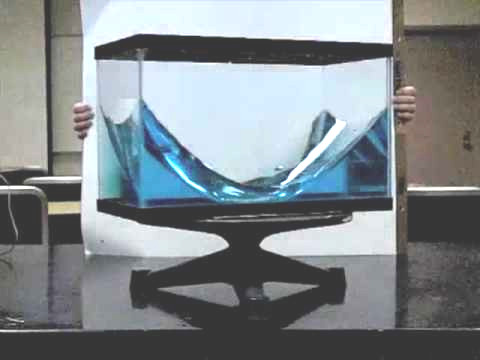
\includegraphics[width=0.5\linewidth]{Figures/Chapter3/fig_water_bucket.jpg}
\caption{A tank of water is smoothly spun up, causing the water to ``climb'' the sides of the tank.  From Dan Russell (\url{https://www.youtube.com/watch?v=Zip9ft1PgV0}).}
\label{fig_bucket}
\end{figure}

Well, the thing that all fluid elements along the free surface have in common is that they have the same pressure -- namely, since they're at the surface, atmospheric pressure $p_0$.  Let's find the pressure in the water, then.

To do that, we'll use Euler's equation, since the flow must satisfy that.  The $x$ component of equation (\ref{eq_euler}) (or the ``$u$'' component), with $\mathbf{g} = [0,0,-g]$, is
\[
\frac{\partial u}{\partial t} + u\frac{\partial u}{\partial x} +  v\frac{\partial u}{\partial y} + w\frac{\partial u}{\partial z} = -\frac{1}{\rho} \frac{\partial p}{\partial x}.
\]
But the flow is \emph{steady}, and $u$ doesn't depend on $x$ or $z$.  Substituting in the fluid velocity in equation (\ref{eq_bucket_vel}), this equation reduces to
\begin{equation}
\label{eq_px}
\frac{\partial p}{\partial x} = \rho \Omega^2 x.
\end{equation}
Similarly, the $v$ and $w$ equations reduce to
\begin{equation}
\label{eq_py}
\frac{\partial p}{\partial y} = \rho \Omega^2 y
\end{equation}
and
\begin{equation}
\label{eq_pz}
\frac{\partial p}{\partial z} = -\rho g.
\end{equation}

We can integrate to find the pressure $p(x, y, z)$.  From equation (\ref{eq_px}) we get
\[
p = \tfrac{1}{2} \rho \Omega^2 x^2 + f(y, z),
\]
where the function $f(yz)$ is there since equation (\ref{eq_px}) is a \emph{partial} derivative -- we don't just get a constant of integration, but a possible function of the other two variables.  Integrating equation (\ref{eq_py}) gives
\[
p = \tfrac{1}{2} \rho \Omega^2 y^2 + g(x, z),
\]
and integrating equation (\ref{eq_pz}) gives
\[
p = -\rho g z + h(x, y).
\]
By inspection, it's clear that the pressure must be
\[
p(x, y, z) = \tfrac{1}{2} \rho \Omega^2 (x^2 + y^2) - \rho gz + p_1,
\]
where $p_1$ is a constant -- it's the pressure at the origin.

That's the pressure everywhere in the water.  To find the shape of the free surface, we'll set $p = p_0$ and solve for the height $z$:
\begin{equation}
z = \frac{\Omega^2}{2g} (x^2 + y^2) + \left( \frac{p_1 - p_0}{\rho g} \right).
\end{equation}
This is a \emph{paraboloid} -- see Fig. \ref{fig_bucket_para} -- and it matches the shape in the photograph in Figure \ref{fig_bucket}.

\begin{figure}
\centering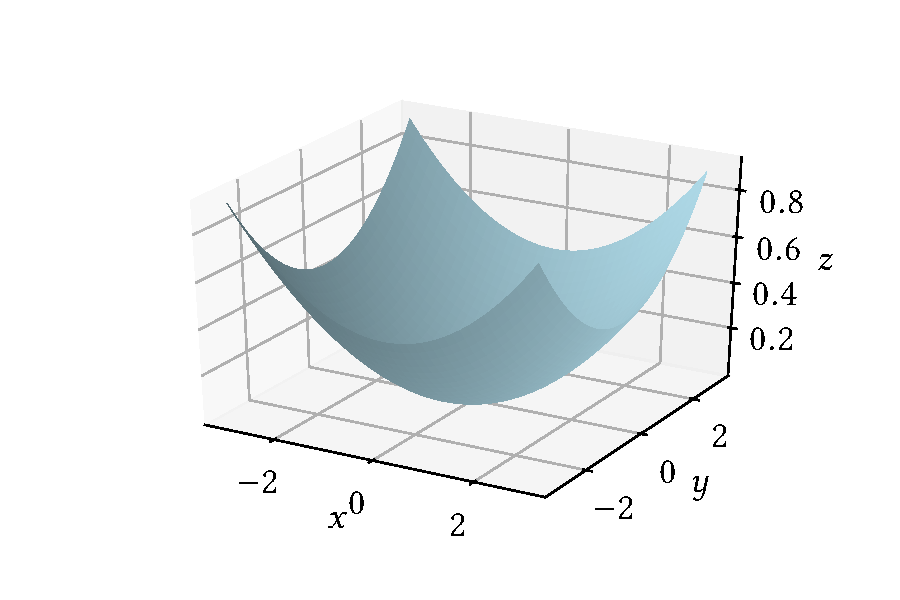
\includegraphics[width=0.8\linewidth]{Figures/Chapter3/fig_paraboloid}
\caption{The free surface of the spinning bucket problem is a paraboloid.}
\label{fig_bucket_para}
\end{figure}





\section{The Velocity Potential and Laplace's Equation}

For any irrotational flow, where
\[
\curl \uu = 0,
\]
a scalar function $\phi$ can be defined such that
\begin{equation}
\label{eq_vel_pot}
\boxed{
\uu = \grad \phi.
}
\end{equation}
Then, since the curl of a gradient is zero, irrotationality is automatically satisfied.  Here, $\phi$ is called the \emph{velocity potential}.

Alternatively, we could write the potential as
\begin{equation}
\label{eq_vel_pot2}
\phi = \int_\mathcal{O}^\mathcal{P} \uu \cdot d\mathbf{x},
\end{equation}
where $\mathcal{O}$ is an arbitrary point in the fluid.  There's a subtle point here, though, so be careful.  As long as the region is \emph{simply connected} -- that is, the fluid has no holes in it -- the path between $\mathcal{O}$ and $\mathcal{P}$ doesn't matter, and $\phi$ will be a single-valued function.

However, if the region is \emph{multiply connected} -- it has holes, regions where there is no fluid -- the integral \emph{could} depend on the path and $\phi$ will be a multivalued function of position.  Let's do some examples to investigate this in detail.

\begin{example}[Uniform flow]
\label{ex_uniform}
Let's start with uniform flow, which is simple and one we'll use extensively. Suppose $\uu = (U, 0, 0)$, where $U$ is the constant velocity of the flow in the $x$-direction. Using either equation (\ref{eq_vel_pot}) or (\ref{eq_vel_pot2}), we can see that
\begin{equation}
\phi = Ux = U r\cos \theta.
\end{equation} 
I've written the potential down in both Cartesian coordinates and also cylindrical; we'll need the cylindrical version later on.
\end{example}

\begin{example}[Flow past a stagnation point]
Recall the flow past a stagnation point, given by
\[
\uu = (\alpha x, -\alpha y, 0).
\]
This is irrotational flow (check if you want!), and to find the velocity potential, write
\[
\frac{\partial \phi}{\partial x} = u = \alpha x \quad \text{and} \quad \frac{\partial \phi}{\partial y} = v = -\alpha y.
\]
Integrating and combining suggests
\[
\phi(x, y) = \tfrac{1}{2} \alpha (x^2 - y^2) + c,
\]
where $c$ is the integration constant.  Note, however, that the fluid velocity, as opposed to the potential, is the physically meaningful quantity; since we take a derivative to get to the velocity, we can set the constant $c$ to zero without worry that it's meaningful.

Note that here $\phi$ is a single-valued function of $x$ and $y$.  That means that, for any point in the fluid, $\phi$ has a single value.
\end{example}

\begin{example}[Line vortex flow]
For our last example, consider the flow
\[
\uu = \frac{k}{r} \, \hat{\theta}.
\]
We have to be careful for this flow -- it's irrotational (we showed that back in Problem \ref{prob_vortex_vorticity}), but not at the origin where it blows up.  To fix this problem, we'll suppose there's \emph{no} fluid there -- maybe there's a cylinder of radius $a$ there instead, covering up the problem area.  That means the fluid domain is $r \ge a$, but it also means there's now a hole in the fluid domain; it's multiply connected.

The potential is found from equation (\ref{eq_vel_pot}) in cylindrical coordinates,
\[
\frac{\partial \phi}{\partial r} = u_r = 0, \quad \frac{1}{r} \frac{\partial \phi}{\partial \theta} = u_\theta = \frac{k}{r}, \quad \text{and} \quad \frac{\partial \phi}{\partial z} = u_z = 0.
\]
Integrating this gives
\begin{equation}
\phi(\theta) = k \theta.
\end{equation}
But note that this isn't a single-valued function -- $\phi$ has different values at the same point in space:  $\phi(0) = 0$, but $\phi(2\pi) = 2\pi k$, and so on.  We'll see later on that this is connected to \emph{circulation} within the fluid.

\end{example}

One final thing before we do one more example.  If the fluid is incompressible, it must satisfy the incompressibility condition,
\[
\div \uu = 0.
\]
If we rewrite this in terms of the potential, we get
\[
\div \grad \uu = 0,
\]
or
\begin{equation}
\boxed{
\nabla^2 \phi = 0.
}
\end{equation}
This is \emph{Laplace's equation}; any irrotational, incompressible fluid must satisfy it.





\section{Example: Flow Past a Cylinder}
\label{sec_cylinder}

For our last example, we'll tackle a more difficult problem -- the ideal flow past a cylinder oriented perpendicular to the flow.

We'll start with a few basic assumptions.  First, this will be treated as two dimensional flow, which means the cylinder is effectively infinitely long.  We'll put the cylinder, which has a radius $a$, along the $z$-axis, and the flow will be uniform in the $x$-direction infinitely far away from the cylinder (see Fig. \ref{fig_cyl_setup}):
\begin{equation}
\label{eq_uniform}
\uu (r \to \infty) = (U, 0, 0),
\end{equation}
where $U$ is the constant speed of the flow far away from the cylinder.

\begin{figure}
\centering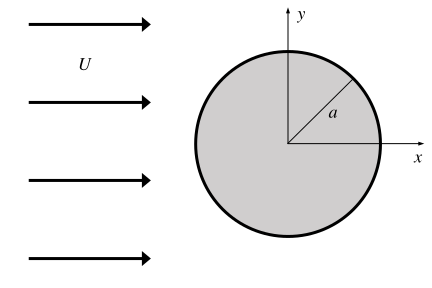
\includegraphics[width=0.7\linewidth]{Figures/Chapter3/fig_cyl_setup}
\caption{Fluid flows past the cylinder along the $x$-direction.}
\label{fig_cyl_setup}
\end{figure}

The other assumption we'll make is that the flow is irrotational.  This seems like a leap to make, though, since we don't even know what the flow \emph{is} yet.  But remember the vorticity equation (\ref{eq_vorticity}) -- for a steady two dimensional flow, the vorticity is conserved along streamlines.  Since the vorticity at infinity, where the flow is \emph{uniform}, is definitely zero, and every streamlines starts and ends at infinity, it follows that the flow is everywhere irrotational.

Wait, is our flow \emph{steady}?  Yes, as long as we examine the problem from the point of view of the flow already happening for a while; it's reached a steady state.  In practice, it doesn't take long for the fluid to do this.

To find the fluid velocity around the cylinder, we'll solve Laplace's equation.  It makes sense to use cylindrical coordinates here, given the symmetry of the boundary.  In cylindrical coordinates, then, Laplace's equation is
\begin{equation}
\label{eq_laplace_cyl}
\ddfdx{\phi}{r} + \frac{1}{r} \dfdx{\phi}{r} + \frac{1}{r^2} \ddfdx{\phi}{\theta} + \ddfdx{\phi}{z} = 0.
\end{equation}
Now, this is an example of two dimensional flow, so the $z$ term we can safely ignore.

Our boundary conditions are straightforward to write down.  First, at $r \to \infty$, we should have the uniform flow given by equation (\ref{eq_uniform}); we found the potential corresponding to this flow in Example \ref{ex_uniform}:
\begin{equation}
\label{eq_cyl_bc1}
\phi = Ur \cos \theta \quad  \text{as} \quad r \to \infty.
\end{equation}
Secondly, at $r=a$, we have the actual boundary.  Unlike viscous flows, ideal fluids must ``slip'' along a boundary; in this case, that means we must have the fluid velocity at $r=a$ be purely in the $\hat{\theta}$ direction.  In other words, we need $u_r = 0$; in terms of the potential (using the gradient in cylindrical coordinates), that's
\begin{equation}
\label{eq_cyl_bc2}
\dfdx{\phi}{r} = 0 \quad \text{at} \quad r=a.
\end{equation}

We'll solve Laplace's equation using separation of variables.  Let
\[
\phi(r, \theta) = R(r) \Theta(\theta).
\]
Then equation (\ref{eq_laplace_cyl}) becomes
\[
\Theta \frac{d^2R}{dr^2} + \frac{\Theta}{r} \frac{dR}{dr} + \frac{R}{r^2} \frac{d^2 \Theta}{d\theta^2} = 0,
\]
or, dividing by $R\Theta$ and multiplying by $r^2$,
\begin{equation}
\label{eq_cyl_sep}
\frac{r^2}{R} \frac{d^2R}{dr^2} + \frac{r}{R} \frac{dR}{dr} = -\frac{1}{\Theta} \frac{d^2 \Theta}{d \theta^2}.
\end{equation}
The left hand side of the equation is a function of $r$ only, while the right hand side is a function of $\theta$ only; they must therefore both be equal to a constant.  We'll call the this separation constant $k^2$.  The $\theta$ equation is then
\[
\frac{d^2 \Theta}{d\theta^2} = -k^2 \Theta,
\]
which has the solution
\[
\Theta (\theta) = A \sin k\theta + B \cos k\theta.
\]

We can apply our first boundary condition, equation (\ref{eq_cyl_bc1}), right away to eliminate the sine term, since we need only a cosine dependence as $r \to \infty$.  Comparing the form of equation (\ref{eq_cyl_bc1}) with our solution, we furthermore must have $k=1$.  Thus 
\begin{equation}
\Theta(\theta) = B \cos \theta.
\end{equation}

The radial part of equation (\ref{eq_cyl_sep}) (with $k = 1$) now reads
\[
r^2 \frac{d^2R}{dr^2} + r \frac{dR}{dr} - R = 0.
\]
We can solve this by trying a power-law solution of the form $R(r) = r^m$; it turns out that the general solution is
\[
R(r) = Cr + \frac{D}{r}.
\]
But our second boundary condition, equation (\ref{eq_cyl_bc2}), was that the first derivative of the potential goes to zero at $r=a$.  That means
\[
\frac{dR}{dr} = \left( C - \frac{D}{r^2} \right)_{r=a} = 0,
\]
and so $D = a^2 C$.

Combining the radial and angular equations gives us
\[
\phi(r, \theta) = R(r) \Theta(\theta) = F \left( r+\frac{a^2}{r} \right) \cos \theta,
\]
where $F=CB$ is our last remaining constant.  One more comparison with our boundary condition, equation (\ref{eq_cyl_bc1}), tells us that $F = U$.  So our solution to Laplace's equation is, finally, 
\begin{equation}
\phi(r, \theta) = U \left( r+\frac{a^2}{r} \right) \cos \theta.
\end{equation}

That's the potential; what about the fluid velocity?  No problem:
\[
\uu = \grad \phi,
\]
so
\begin{equation}
u_r(r, \theta) = U \left( 1 - \frac{a^2}{r^2} \right) \cos \theta
\end{equation}
and
\begin{equation}
u_\theta(r, \theta) = -U \left( 1 + \frac{a^2}{r^2} \right) \sin \theta.
\end{equation}
From $\uu$, we can sketch streamlines, which are shown in Figure \ref{fig_cyl_streamlines}.

\begin{figure}
\centering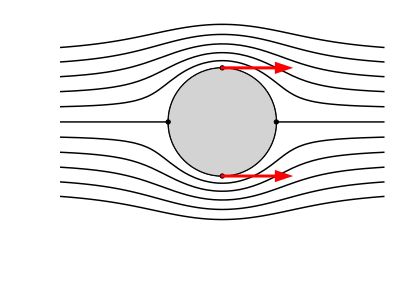
\includegraphics[width=0.7\linewidth]{Figures/Chapter3/fig_cylinder_stream}
\caption{The streamlines for the flow around the cylinder.  Note that there are stagnation points upstream and downstream of the cylinder ($\theta = 0$ and $\theta = \pi$), and the fluid has greatest velocity at the top and bottom ($\theta = \pi2$ and $\theta = 3\pi/2$).}
\label{fig_cyl_streamlines}
\end{figure}

Let's examine the flow in a little more detail.  Note that, as necessary, $u_r=0$ at $r=a$.  On the boundary, the flow is purely angular, with speed 
\[
u_\theta = -2U \sin \theta \quad \text{at} \quad r=a.
\]
At $\theta = 0$ and $\theta = \pi$, then $u_\theta = 0$ and there is a stagnation point there (see Figure \ref{fig_cyl_streamlines}).  There is a maximum speed at $\theta = \pi/2$ and $\theta = 3\pi/2$ of
\[
u_{\theta, \text{max}} = 2U \quad \text{at} \quad r=a.
\]

What about the pressure in the fluid?  Well, we could apply Euler's equation to find it, but Bernoulli's principle provides a shortcut.  Since the flow is irrotational, $\grad H = 0$ and $H = p/\rho + \tfrac{1}{2} \uu^2 + gz = $ constant everywhere in the fluid.  In our analysis, though, we'll neglect the gravity term; we're only looking at the $(r, \theta)$ dependence of the pressure here, and gravity will only impose an overall vertical pressure gradient.

Let's first evaluate $H$ at infinity, where $\uu = (U,0,0)$ and we'll label the pressure $p_\infty$.  Then
\[
H = \frac{p_\infty}{\rho} + \tfrac{1}{2} U^2.
\]
Elsewhere in the fluid, it's
\[
H = \frac{p(r, \theta)}{\rho} + \tfrac{1}{2} \uu^2,
\]
where
\[
\uu^2 = \uu \cdot \uu = u_r^2 + u_\theta^2 = U^2 \left( 1 + \frac{a^4}{r^4} - 2\frac{a^2}{r^2} \cos 2\theta \right)
\]
(that last step required some algebra to clean up, though).  Since $H$ is constant, we have
\[
\frac{p(r, \theta)}{\rho} + \tfrac{1}{2} U^2 \left( 1 + \frac{a^4}{r^4} - 2\frac{a^2}{r^2} \cos 2\theta \right) = \frac{p_\infty}{\rho} + \tfrac{1}{2} U^2.
\]
Rearranging gives the pressure,
\begin{equation}
p(r, \theta) = p_\infty + \tfrac{1}{2} \rho \frac{a^2}{r^2} U^2 \left( 2 \cos 2\theta - \frac{a^2}{r^2} \right).
\end{equation}
Figure \ref{fig_cyl_pressure} shows the pressure around the cylinder; there is a region of high pressure at $\theta = 0$ and $\theta = \pi$, with low pressure at $\theta = \pi/2$ and $\theta = 3\pi/2$.  Not surprisingly, this is opposite the fluid velocity -- expected, since Bernoulli's theorem holds here.

\begin{figure}[t]
\centering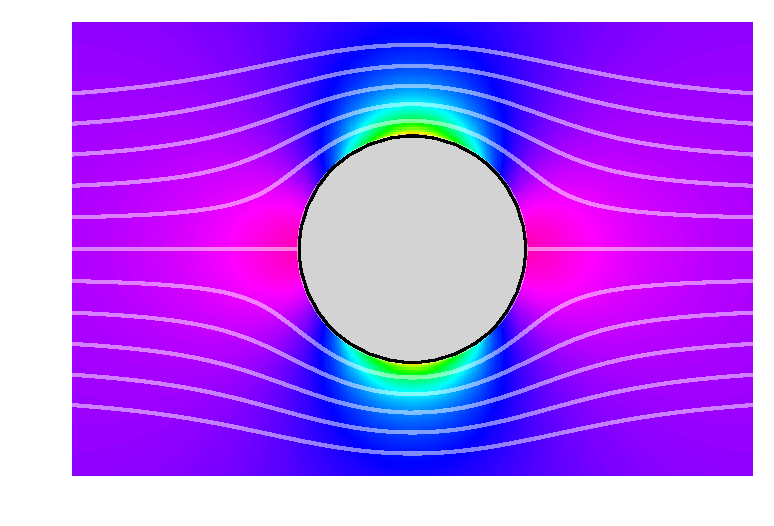
\includegraphics[width=0.8\linewidth]{Figures/Chapter3/fig_cylinder_pressure}
\caption{The pressure field of fluid flowing past a cylinder.  The pinkish regions are areas of high pressure, while the yellow/green areas are low pressure.  The streamlines are shown as well.}
\label{fig_cyl_pressure}
\end{figure}








\section*{Problems}
\addcontentsline{toc}{section}{Problems}

\begin{problem}[Yet more vector calculus]
\label{prob_vc3}
Show that, for any vector field $\mathbf{v}$, you can write
\[
(\mathbf{v} \cdot \grad ) \mathbf{v} = (\curl \mathbf{v}) \times \mathbf{v} + \grad(\tfrac{1}{2} \mathbf{v}^2).
\]
\end{problem}

\begin{problem}[Please, no more vector calculus]
\label{prob_vc4}
Show that, for any two vector fields $\mathbf{F}$ and $\mathbf{G}$, you can write
\[
\curl (\mathbf{F} \times \mathbf{G}) = (\mathbf{G} \cdot \grad) \mathbf{F} - (\mathbf{F} \cdot \grad) \mathbf{G} + \mathbf{F} (\div \mathbf{G}) - \mathbf{G} (\div \mathbf{F})
\]
\end{problem}


\begin{problem}[The Rankine Vortex as a Model for Hurricanes]
A Rankine vortex is defined by the flow (in cylindrical coordinates)
\[
\mathbf{u}  = \left\{
 \begin{array}{l l}
    \Omega r \, \hat{\theta} & \quad \text{if $r < a$}\\
   \frac{\Omega a^2}{r} \, \hat{\theta} & \quad \text{if $r>a$,}
  \end{array} \right.
\]
where $\Omega$ and $a$ are constants (related to the wind speed and size of the ``core,'' respectively).  It serves as a useful model for a number of weather and atmospheric conditions, such as hurricanes, mesocyclones, and tornadoes.  

(a) Plot the wind speed as a function of distance, and calculate and plot the vorticity.

(b) To decide whether it is a useful model for hurricanes, I've provided (online) azimuthal wind speed data and vorticity data for Hurricane Katrina, which devastated New Orleans and the surrounding area in 2005.  The wind speed data has the first column as distance $r$ (in km) and the second column as azimuthal wind speed $u_\theta$ (in m/s).  The vorticity data has the first column as distance $r$ (in km) and the second column as vorticity $\omega$ (in $10^{-4}$ s$^{-1}$).

Use the Rankine vortex (RV) to model this hurricane; what values of $\Omega$ and $a$ give you the best fit?  Does the RV model the vorticity with those parameters as well?  Can you make any conclusions about how well the model does (e.g., is it better in some regions versus others?)

(c) Calculate the pressure throughout the hurricane and find the difference in pressure between r = 0 (the eye of the hurricane) and $r \to \infty$ (outside the storm).

(d) Finally, calculate the shape of the free surface (i.e., where the pressure is atmospheric). Plot the surface as a 3D surface. Compare this with photos of Katrina -- how does it look?
\end{problem}



\begin{problem}[The force on a cylinder]
We've already calculated the pressure in the fluid around a cylinder in Section \ref{sec_cylinder}, so it's a short leap to find the total force exerted on the cylinder by the fluid.

Consider Figure \ref{fig_cylinder_force}:  the force (per unit length of the cylinder) on a small angular section of size $a \, d\theta$ is
\[
d\textbf{F} = - p \hat{n}.
\]
Using this, show the total force on the cylinder is zero.  This is called \emph{D'Alembert's paradox} -- there's no drag on the cylinder, despite very obvious physical evidence to the contrary.  Does it make sense that the fluid exerts no force at all on the cylinder as it flows past?  Discuss this a bit.

\begin{figure}[t]
\centering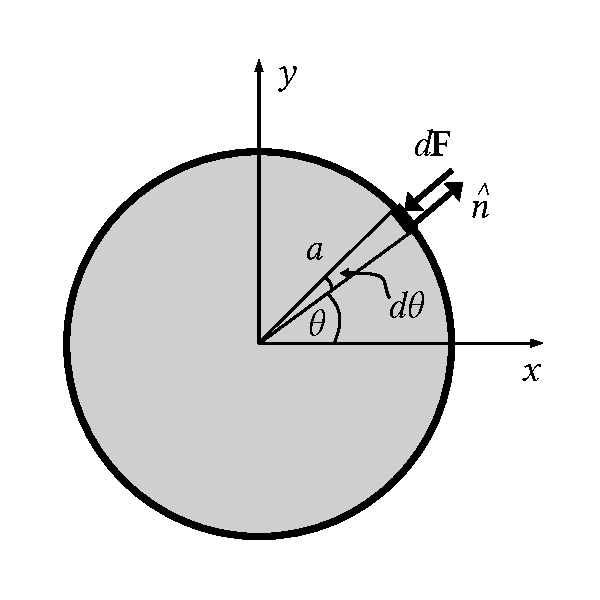
\includegraphics[width=0.5\linewidth]{Figures/Chapter3/fig_cyl_force}
\caption{The force on a small angular section of the cylinder.  The force is opposite the normal vector $\hat{n}$.}
\label{fig_cylinder_force}
\end{figure}

\end{problem}
